\section{1D Navier-Stokes Equations}
\subsection{Derivation}
Starting with the 2D Navier-Stokes (NS) Equations, namely
\begin{subequations}
    \begin{equation}
        \pdv{u}{t} + \pdv{uu}{x} + \pdv{uv}{y} = 
                -\frac{1}{\rho} \pdv{p}{x} 
                + \nu \left( \pdv{u}{x}{x} + \pdv{u}{y}{y} \right) 
        \label{eq:NS-u}
    \end{equation}
    \begin{equation}
        \pdv{v}{t} + \pdv{uv}{x} + \pdv{vv}{y} = 
                -\frac{1}{\rho} \pdv{p}{y} 
                + \nu \left( \pdv{v}{x}{x} + \pdv{v}{y}{y} \right) 
        \label{eq:NS-v}
    \end{equation}
\end{subequations}
where for 1D all the gradients in the $x$-direction are zero 
($\pdv*{(\;)}{x}=0$), reducing Eqs.~(\ref{eq:NS-u},\ref{eq:NS-v}) to
\begin{subequations}
    \begin{equation}
        \pdv{u}{t} + \pdv{uv}{y} = 
            -\frac{1}{\rho} \pdv{p}{x}
            + \nu \pdv{u}{y}{y}
        \label{eq:NS-u-1d}
    \end{equation}
    \begin{equation}
        \pdv{v}{t} + \pdv{vv}{y} =
            -\frac{1}{\rho} \pdv{p}{y} +  
            \nu \pdv{v}{y}{y}
        \label{eq:NS-v-1d}
    \end{equation}
\end{subequations}
Next, we recognize that the transport of $v$ is independent of $u$,
therefore a solution of $v(y,t)$ can be obtained solely from
Eq.~(\ref{eq:NS-v-1d}) and be substituted into Eq.~(\ref{eq:NS-u-1d}) to
determine $u(y,t)$.  Similarly to solving the 2D-NS equations, we can apply
the fractional step method and separate Eq.~(\ref{eq:NS-v-1d}) into the
following steps 
\begin{subequations}
    \begin{equation}
        \pdv{v}{t} =  - \pdv{vv}{y} + \nu \pdv{v}{y}{y} 
        \hspace{0.25cm}
        : v^{n} \rightarrow v^{\ast}
        \label{eq:NS-un-1d}
    \end{equation}
    \begin{equation}
        \pdv{v}{t} = -\frac{1}{\rho} \pdv{p}{y}
        \hspace{0.25cm}
        : v^{\ast} \rightarrow v^{n+1}
        \label{eq:NS-ustar-1d}
    \end{equation}
\end{subequations}
Additionally the pressure is calculated using the divergence of
Eq.~(\ref{eq:NS-ustar-1d}) and applying the continuity equation, namely  
\begin{subequations}
    \begin{align}
        -\frac{1}{\rho} \text{div}(\text{grad}(p)) & =
                \text{div}\bigg(\pdv{v}{t}\bigg)        \\
        -\frac{1}{\rho} \text{div}(\text{grad}(p)) & =
            \frac{
                    \cancel{\text{div}\big(v^{n+1}_{j+\frac{1}{2}}\big)} -
                    \text{div}\big(v^{\ast}_{j+\frac{1}{2}}\big)
                }
                {\Delta t}
    \end{align}
\end{subequations}
Thus
\begin{equation}
    -\frac{1}{\rho} \text{div}(\text{grad}(p)) =
        \frac{1}{\Delta t} \text{div} \big(v^{\ast}_{j+\frac{1}{2}}\big)
\end{equation}
\newpage
\subsection{Finite Difference Equations}
Discretetizing the above equations on a staggered grid shown in
Fig.~(\ref{fig:1d-grid}) gives the following finite difference formulas,
starting with Eq.~(\ref{eq:NS-un-1d})

\begin{subequations}
    \colorboxed{
        v^{\ast}_{j+\frac{1}{2}} = v^{n}_{\frac{1}{2}} 
                                -\Delta t \frac{\left(v^{n}_{j+1}\right)^{2}-\left(v^{n}_{j}\right)^{2}}
                                    {\Delta y}
                                +\nu \Delta t \
                                \frac{v^{n}_{j+\frac{3}{2}}-2v^{n}_{j+\frac{1}{2}}+v^{n}_{j-\frac{1}{2}}}
                                    {\Delta y^{2}}
            }
    \text{where}
    \colorboxed{
        v^{n}_{j+1} = \frac{1}{2} \left(v^{n}_{j+\frac{3}{2}} + v^{n}_{j+\frac{1}{2}}\right) 
        }
    \colorboxed{
        v^{n}_{j} = \frac{1}{2} \left(v^{n}_{j+\frac{1}{2}} + v^{n}_{j-\frac{1}{2}}\right) 
    }
\end{subequations}
Furthermore, the pressure is obtained by solving the following Poisson equation using a tri-diagonal
solver,
\colorboxed{
    \frac{1}{\rho} \left( \frac{p_{i+1} -2 p_{i} + p_{i-1}} {\Delta x^2} \right) =
            \frac{1}{\Delta t} \Bigg(\frac{u^{\ast}_{i+\frac{1}{2}} - u^{\ast}_{i-\frac{1}{2}}}
            {\Delta x}  \Bigg)
        }
Moreover, the evolution of $v$ is determined using the following 
\colorboxed{
    v^{n+1}_{j+\frac{1}{2}} = v^{\ast}_{j+\frac{1}{2}} - \Delta t \left(\frac{p_{j+1} - p_{j}}{\Delta y}\right) 
    }
Lastly, $u^{n+1}$ is calculated using $v^{n}$,
\begin{subequations}
    \colorboxed{
        u^{n+1}_{j} = u^{n}_{j} 
                    - \Delta t   \frac{(uv)^{n}_{j+\frac{1}{2}} -(uv)^{n}_{j-\frac{1}{2}}}{\Delta y}
                    + \nu \Delta t \frac{u^{n}_{j+1} - 2u^{n}_{j} + u^{n}_{j-1}}{\Delta y ^{2}}  
                }
    \text{where}
    \colorboxed{
        u^{n}_{j+\frac{1}{2}} = \frac{1}{2}\left(u^{n}_{j+1} + u^{n}_{j}\right)
    }
    \colorboxed{
        u^{n}_{j-\frac{1}{2}} = \frac{1}{2}\left(u^{n}_{j} + u^{n}_{j-1}\right)
    }
\end{subequations}
\begin{figure}[H]
    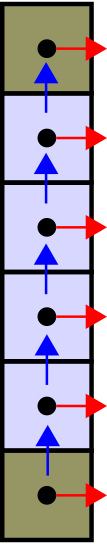
\includegraphics[height=0.5\textheight]{../../media/1d-NS}
    \caption{1D staggered grid}
    \label{fig:1d-grid}
\end{figure}
